\chapter{Opis teoretyczny}
\label{cha:opis_teor}

\section{Gra}
\label{sec:gra}
W niniejszej pracy będziemy skupiali się na grach 3 oraz N-osobowych. Będziemy rozpatrywać tylko przypadki w których koalicja dwóch graczy wygrywa. Nie bierzemy pod uwagę sytuacji w których współpraca ze sobą wszystkich graczy mogłaby przynieść najlepsze korzyści. W tabelce wypłat rozważanej gry nie może pojawić się punkt równowagi wynikający ze strategii czystych. W rozważane przez nas grze celem gracza nie jest zdobycie jak największego zysku, lecz osiągnięcie jak największej liczby wygranych. Osoba znajdująca się poza koalicją przegrywa i wszyscy gracze mają taką samą wagę wyboru. Model gry 3-osobowej pokazuje nam, że decyzję jednego z zawodników mają bezpośredni wpływ na zachowanie sąsiadów. W modelu gry N-osobowej decyzje graczy będą propagowane na kolejne lokalne gry 3-osobowe, co będzie pośrednio wpływać na decyzję graczy w sąsiednich rozgrywkach.

Omawiane tutaj gry są grami o niepełnej informacji. Najłatwiej to wyjaśnić opisując grę o pełnej informacji, czyli taką której:
\begin{itemize}
\item żaden z węzłów nie jest przypisany losowi
\item każdy węzeł należy do osobnego zbioru informacji
\end{itemize}
Drzewko gry wizualizuję rozgrywkę analogicznie jak drzewko prawdopodobieństwa mogłoby pokazać wszystkie scenariusze rzutu 3 kostkami z rzędu. Jest to definicja która jest najczęściej używana, lecz my potrzebujemy innej. Jest to spowodowane tym, że omawiana przez nas gra nie jest sekwencyjna i nie możemy do niej użyć drzewka gry. W tej pracy przez grę o pełnej informacji będziemy rozumieli grę, w której wszyscy uczestnicy znają prawdopodobieństwo wyborów przeciwników, co nie jest prawdą w naszym przypadku.

\section{Model gry}
W niniejszej pracy będziemy potrzebowali dwóch modeli gier. Pierwszym z nich będzie model gry 3-osobowej \ref{fig:model_niezal}. Zacznijmy od nazwania graczy odpowiednio $G_0$, $G_1$, $G_2$ (gracz pierwszy, drugi, trzeci). Każdy z nich posiada prawdopodobieństwo zagrania na gracza o wyższym indeksie (zapętlamy dla trzeciego gracza) $p_i$. Prawdopodobieństwo zagrania na gracza o niższym indeksie (zapętlamy dla pierwszego gracza) wynosi $1 - p_i$ i nie musi być przechowywane, ponieważ możemy to w łatwy sposób wyliczyć. Ponadto są one dostępne tylko dla graczy, których opisują. Żaden z zawodników nie ma dostępu do prawdopodobieństw innych graczy, lecz każdy ma dostęp do statystyki gry na którą składa się:
\begin{itemize}
\item $liczba_{partii}$ liczba rozegranych w grze partii
\item $nast_i$ ilość zagrań $G_i$ na gracza $G_{i+1}$, ilość zagrań na $G_{i-1}$ możemy wziąć z $liczba_{partii} - nast_i$
\end{itemize}
Drugi z modeli \ref{fig:model_zal} będzie się nieznacznie różnił. Będzie to gra N-osobowa składająca się z lokalnych gier 3-osobowych. Pozostała cześć modelu się nie zmienia.
{\color{red} UKŁAD}
\begin{figure}
	\centering
	\begin{tabular}{c|c}
	\subfloat[3-osobowej \label{fig:model_niezal}]{ 
		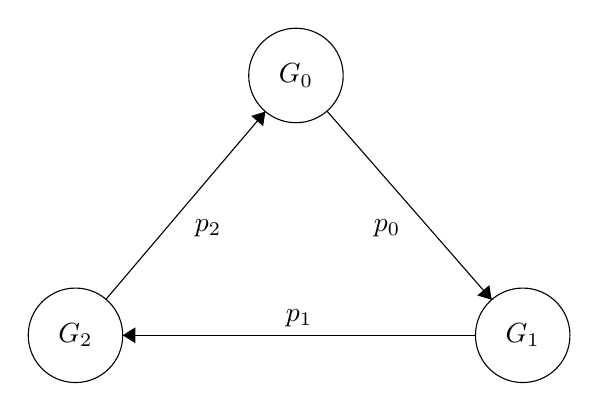
\begin{tikzpicture}[scale=0.2]
		\tikzstyle{every node}+=[inner sep=0pt]
		\draw [black] (40.6,-18.2) circle (3);
		\draw (40.6,-18.2) node {$G_0$};
		\draw [black] (55,-34.7) circle (3);
		\draw (55,-34.7) node {$G_1$};
		\draw [black] (26.6,-34.7) circle (3);
		\draw (26.6,-34.7) node {$G_2$};
		\draw [black] (42.57,-20.46) -- (53.03,-32.44);
		\fill [black] (53.03,-32.44) -- (52.88,-31.51) -- (52.12,-32.17);
		\draw (47.26,-27.9) node [left] {$p_0$};
		\draw [black] (52,-34.7) -- (29.6,-34.7);
		\fill [black] (29.6,-34.7) -- (30.4,-35.2) -- (30.4,-34.2);
		\draw (40.8,-34.2) node [above] {$p_1$};
		\draw [black] (28.54,-32.41) -- (38.66,-20.49);
		\fill [black] (38.66,-20.49) -- (37.76,-20.77) -- (38.52,-21.42);
		\draw (34.15,-27.89) node [right] {$p_2$};
		\end{tikzpicture}
	} &
	\subfloat[N-osobowej \label{fig:model_zal}]{  
		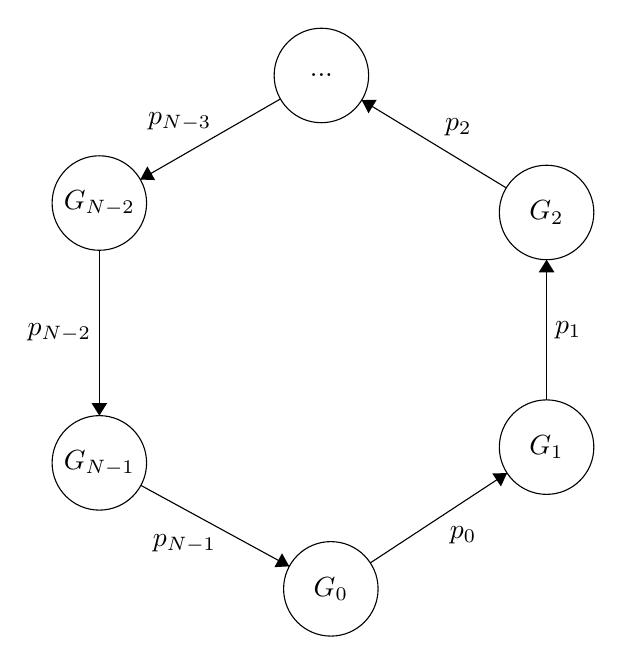
\begin{tikzpicture}[scale=0.2]
		\tikzstyle{every node}+=[inner sep=0pt]
		\draw [black] (38.2,-44.1) circle (3);
		\draw (38.2,-44.1) node {$G_0$};
		\draw [black] (51.9,-35.1) circle (3);
		\draw (51.9,-35.1) node {$G_1$};
		\draw [black] (23.5,-36.1) circle (3);
		\draw (23.5,-36.1) node {$G_{N-1}$};
		\draw [black] (51.9,-20.2) circle (3);
		\draw (51.9,-20.2) node {$G_2$};
		\draw [black] (23.5,-19.6) circle (3);
		\draw (23.5,-19.6) node {$G_{N-2}$};
		\draw [black] (37.6,-11.5) circle (3);
		\draw (37.6,-11.5) node {$...$};
		\draw [black] (40.71,-42.45) -- (49.39,-36.75);
		\fill [black] (49.39,-36.75) -- (48.45,-36.77) -- (49,-37.6);
		\draw (46.6,-40.1) node [below] {$p_0$};
		\draw [black] (26.14,-37.53) -- (35.56,-42.67);
		\fill [black] (35.56,-42.67) -- (35.1,-41.84) -- (34.62,-42.72);
		\draw (28.91,-40.6) node [below] {$p_{N-1}$};
		\draw [black] (23.5,-22.6) -- (23.5,-33.1);
		\fill [black] (23.5,-33.1) -- (24,-32.3) -- (23,-32.3);
		\draw (23,-27.85) node [left] {$p_{N-2}$};
		\draw [black] (51.9,-32.1) -- (51.9,-23.2);
		\fill [black] (51.9,-23.2) -- (51.4,-24) -- (52.4,-24);
		\draw (52.4,-27.65) node [right] {$p_1$};
		\draw [black] (49.34,-18.64) -- (40.16,-13.06);
		\fill [black] (40.16,-13.06) -- (40.59,-13.9) -- (41.11,-13.05);
		\draw (46.3,-15.35) node [above] {$p_2$};
		\draw [black] (35,-12.99) -- (26.1,-18.11);
		\fill [black] (26.1,-18.11) -- (27.04,-18.14) -- (26.55,-17.27);
		\draw (28.6,-15.05) node [above] {$p_{N-3}$};
		\end{tikzpicture}
	}
	\end{tabular}
\caption{Modele gry}
\label{fig:modele}
\end{figure}

Wszystkie zmiany prawdopodobieństwa muszą przejść funkcję ograniczającą, więcej o niej znajdziemy w sekcji \ref{sec:ograniczenie}. Jak uzyskać $\Delta p_i$ dowiemy się w dwóch następnych podrozdziałach.
\begin{equation} \label{eq:ograniczenie}
p_i = ogr( p_i + \Delta p_i)
\end{equation}
%---------------------------------------------------------------------------------------------------------------------------------------------------------------------

\section{Równania standardowe}
\label{sec:r_stand}
Podstawowym równaniem od którego wyjdziemy będzie równanie dla gracza o indeksie 0, pozostałe utworzymy analogicznie:
{\color{red} SKĄÐ}
\begin{equation} \label{eq:poczatek}
\Delta p_0 = (1 - p_1) - p_2
\end{equation}
Człon $1 - p_1$ jest prawdopodobieństwem zagrania gracza 1 na gracza 0, więc prawdopodobieństwo zagrania gracza 0 na gracza 1 powinno z nim rosnąć. Zniechęcić gracza 0 do sympatyzowania z graczem 1 mogłyby zagrania gracza 2 w kierunku gracza 3. Z tego właśnie powodu odejmujemy $p_2$, co ma pokazywać graczowi 0 że ma innego zawodnika, który wyciąga do niego rękę.

Z powodu że mamy do czynienia z grą o niepełnej informacji zdecydowałem się wprowadzić u zawodników statystykę zagrań przeciwników, pozwalającą obliczyć prawdopodobieństwo. W jednej z następnych sekcji \ref{sec:ograniczenie} omówimy bardziej szczegółowo niechciane zachowania z tego wynikające, ale na chwilę obecną przyjmijmy, że potrzebujemy dodatkowego parametru $\alpha$ przyjętego na poziomie $0.1$.

W poniższym równaniu $n_N$ oznacza liczbę partii zagranych przez następnego (z wyższym indeksem) gracza w kierunku jego następnego gracza. Analogicznie $n_P$ oznacza liczbę partii zagranych przez poprzedniego (z niższym indeksem) gracza w kierunku jego następnego gracza (czyli nas).
\begin{equation} \label{eq:stand}
\Delta p_i = \alpha \cdot (1 - \frac{n_N}{liczba_{partii}} - \frac{n_P}{liczba_{partii}})
\end{equation}

%---------------------------------------------------------------------------------------------------------------------------------------------------------------------

\section{Równania replikatorów}
\label{sec:r_repli}
Model dynamiki replikatorów jest najbardziej znanym różniczkowym modelem teorii gier ewolucyjnych, przez co może stanowić dobry wybór do sterowania zachowaniem graczy. Tak jak w poprzednim przypadku przyjmijmy prawdopodobieństwa kolejno $x$, $y$ oraz $z$ pamiętając, że prawdopodobieństwa poza tym z pochodnej są szacowane. Podstawowy wzór równania wygląda następująco:
\begin{equation}
\dot{x} = x \cdot ( W - \overline{W})
\end{equation}
Gdzie $W$ jest średnią wypłatą dla strategii $x$ (dla nas prawdopodobieństwem gry na x), natomiast $\overline{W}$ jest średnią wypłatą co daje nam:
{\color{red} UKŁAD}
\begin{align*}
\dot{x} = x \cdot ( \overbrace{(1-y)}^{W} - \overbrace{(x(1-y) + (1-x)z)}^{\overline{W}}) \\
\Downarrow \\
\dot{x} = x \cdot (1-x) \cdot (1-y-z)
\end{align*}
Co dla gry 3-osobowej generuje równania:
\begin{align} \label{eq:repli}
\Delta p_0 = \alpha p_0 \cdot (1 - p_0) \cdot (1 - \frac{n_1}{liczba_{partii}} - \frac{n_2}{liczba_{partii}}) \nonumber \\
\Delta p_1 = \alpha p_1 \cdot (1 - p_1) \cdot (1 - \frac{n_2}{liczba_{partii}} - \frac{n_0}{liczba_{partii}}) \\
\Delta p_2 = \alpha p_2 \cdot (1 - p_2) \cdot (1 - \frac{n_0}{liczba_{partii}} - \frac{n_1}{liczba_{partii}}) \nonumber
\end{align} 

%---------------------------------------------------------------------------------------------------------------------------------------------------------------------

\section{Ograniczenie prawdopodobieństwa}
\label{sec:ograniczenie}
Jak zauważyliśmy powyższe równania w łatwy sposób mogą wyjść poza przedział $<0,1>$. Aby temu zapobiec każda inkrementacja prawdopodobieństwa musi być obłożona funkcją ograniczającą. Każde nowo obliczone prawdopodobieństwo podawane jest jako parametr do funkcji $ogr$, a dopiero jej rezultat jest przypisywany poszczególnym prawdopodobieństwom graczom. Zdecydowałem się użyć następującej funkcji:
\begin{displaymath}
ogr(p_i) = \left\{
\begin{array}{ll}
1 & \text{jeżeli } p_i > 1 \\
p_i & \text{jeżeli } 1 \geq p_i \geq 0 \\
0 & \text{jeżeli } p_i < 0
\end{array} 
\right.
\end{displaymath}

Zapewne naszą uwagę przykuł także parametr $\alpha$ obecny w powyższych równaniach. W pierwszym z nich użycie go jest konieczne, gdyż w przeciwnym przypadku szacowanie prawdopodobieństwa innych doprowadziłoby do zawiązania trwałych koalicji już po pierwszej partii. N oznacza zagranie w stronę zawodnika z wyższym numerem, natomiast P z niższym. Zapętla to się dla pierwszego i ostatniego gracza. Zobaczmy przykład dla równania standardowego, prawdopodobieństwa początkowego $\frac{1}{2}$ i $\alpha = 1$ zakładając że:
\begin{align*}
Gracz_0 = N, Gracz_1 = P, Gracz_2 = N && Gracz_0 = N, Gracz_1 = P, Gracz_2 = P\\
\left\{
\begin{array}{ll}
\Delta p_0 = (1 - 0 - 1) =  0 & p_0=\frac{1}{2}\\
\Delta p_1 = (1 - 1 - 1) =  -1 & p_1= 0\\
\Delta p_2 = (1 - 1 - 0) =  0 & p_2=\frac{1}{2}\\
\end{array} 
\right. &&
\left\{
\begin{array}{ll}
\Delta p_0 = (1 - 0 - \frac{1}{2}) =  0 & p_0=\frac{3}{4}\\
\Delta p_1 = (1 - \frac{1}{2} - 1) =  -\frac{1}{2} & p_1= 0\\
\Delta p_2 = (1 - 0 - \frac{1}{2}) =  \frac{1}{2} & p_2=\frac{3}{4}\\
\end{array}
\right.
\end{align*}
Schemat po lewej przedstawia pierwszą partię, a po lewej drugą. Jak widzimy prowadzi to do bardzo szybkich zmian prawdopodobieństwa, co może praktycznie uniemożliwiać jakiekolwiek zmiany sojuszy. Wartym rozważenia jest czy w równaniach replikatorów potrzebny będzie jakiś parametr zmniejszający dynamikę skoro posiadają człon postaci $x(1-x)$. Weźmy założenia z poprzedniego przykładu. Przeanalizujmy przykład: {\color{red} UKŁAD}
\begin{align*}
Gracz_0 = N, Gracz_1 = P, Gracz_2 = N \\
\left\{
\begin{array}{ll}
\Delta p_0 = \frac{1}{2} \cdot (1 - \frac{1}{2}) \cdot (1 - 0 - 1) =  0 & p_0=\frac{1}{2}\\
\Delta p_1 = \frac{1}{2} \cdot (1 - \frac{1}{2}) \cdot (1 - 1 - 1) =  0 & p_1= \frac{1}{4}\\
\Delta p_2 = \frac{1}{2} \cdot (1 - \frac{1}{2}) \cdot (1 - 0 - 1) =  0 & p_2=\frac{1}{2}\\
\end{array} 
\right.
\\
Gracz_0 = N, Gracz_1 = P, Gracz_2 = P \\
\left\{
\begin{array}{ll}
\Delta p_0 = \frac{1}{2} \cdot (1 - \frac{1}{2}) \cdot (1 - 0 - \frac{1}{2}) = \frac{1}{8} & p_0=\frac{5}{8}\\
\Delta p_1 = \frac{1}{4} \cdot (1 - \frac{1}{4}) \cdot (1 - \frac{1}{2} - 1) = -\frac{1}{32} & p_1= \frac{7}{32}\\
\Delta p_2 = \frac{1}{2} \cdot (1 - \frac{1}{2}) \cdot (1 - 0 - \frac{1}{2}) = \frac{1}{8}  & p_2=\frac{5}{8}\\
\end{array}
\right.
\end{align*}
Jak widzimy najszybsza zmiana zachodzi dla pierwszego gracza, który traci 25\% zaufania do gracza o wyższym indeksie. W kolejnej partii nie widzimy już tak dużych zmian. Należy odpowiedzieć na pytanie czy jest to na tyle dużo, aby wprowadzać parametr mający spowalniać dynamikę zmian. Powinno się poruszyć dwie kwestie. Zgadzam się że dynamika prawdopodobieństwa jest dla mnie akceptowalna(czyli wynosi do 10\%), ale tylko dla prawdopodobieństw które oddalają się od środka przedziału, a grę rozpoczynamy właśnie w nim. Drugą sprawą jest porównanie obu równań. Porównanie wyników, w które rekurencyjnie wkładamy czynnik wymnażający zmianę nie jest najłatwiejszą rzeczą do opisania. Celem członu $x(1-x)$ w równaniu replikatorów jest rozwiązanie problemu supersilnych, szybko tworzących się koalicji.

Postarajmy się teraz skupić na szczególnych przypadkach, gdy w obu osobnych grach żaden z graczy nie współpracował. Użyjemy równań standardowych, prawdopodobieństwo początkowe $\frac{1}{2}$ oraz $\alpha = 1$.

\begin{align*}
Gracz_0 = N, Gracz_1 = N, Gracz_2 = N && Gracz_0 = P, Gracz_1 = P, Gracz_2 = P \\
\left\{
\begin{array}{ll}
\Delta p_0 = (1 - 1 - 1) =  -1 & p_0=0\\
\Delta p_1 = (1 - 1 - 1) =  -1 & p_1= 0\\
\Delta p_2 = (1 - 1 - 1) =  -1 & p_2=0\\
\end{array} 
\right. &&
\left\{
\begin{array}{ll}
\Delta p_0 = (1 - 0 - 0) =  1 & p_0= 1\\
\Delta p_1 = (1 - 0 - 0) =  1 & p_1= 1\\
\Delta p_2 = (1 - 0 - 0) =  1 & p_2= 1\\
\end{array}
\right.
\end{align*}
Przypadek ten pokaże nam skutki braku ograniczenia w prawdopodobieństwie. Wiemy że teraz każdy z graczy wykona ruch przeciwny do poprzedniego co da nam w obu grach:
\begin{align*}
\left\{
\begin{array}{l}
\Delta p_0 = (1 - \frac{1}{2} - \frac{1}{2}) =  0 \\
\Delta p_1 = (1 - \frac{1}{2} - \frac{1}{2}) =  0 \\
\Delta p_2 = (1 - \frac{1}{2} - \frac{1}{2}) =  0 \\
\end{array} 
\right.
\end{align*}
Brak wpływu na zmiany, gracze dokonują wyboru jak poprzednio.
\begin{align*}
Gracz_0 = P, Gracz_1 = P, Gracz_2 = P && Gracz_0 = N, Gracz_1 = N, Gracz_2 = N \\
\left\{
\begin{array}{ll}
\Delta p_0 = (1 - \frac{1}{3} - \frac{1}{3}) =  \frac{1}{3} & p_0= \frac{1}{3}\\
\Delta p_1 = (1 - \frac{1}{3} - \frac{1}{3}) =  \frac{1}{3} & p_1= \frac{1}{3}\\
\Delta p_2 = (1 - \frac{1}{3} - \frac{1}{3}) =  \frac{1}{3} & p_2= \frac{1}{3}\\
\end{array} 
\right. &&
\left\{
\begin{array}{ll}
\Delta p_0 = (1 - \frac{2}{3} - \frac{2}{3}) =  -\frac{1}{3} & p_0= \frac{2}{3}\\
\Delta p_1 = (1 - \frac{2}{3} - \frac{2}{3}) =  -\frac{1}{3} & p_1= \frac{2}{3}\\
\Delta p_2 = (1 - \frac{2}{3} - \frac{2}{3}) =  -\frac{1}{3} & p_2= \frac{2}{3}\\
\end{array}
\right.
\end{align*}
Nie wróciliśmy to punktu wyjścia, w którym wyjściowym prawdopodobieństwem chęci gry na gracza z większym indeksem jest $\frac{1}{3}$ dla gry przedstawionej po lewej stronie i $\frac{2}{3}$ dla gry po prawej. W pamięci każdego z graczy jest liczba rozegranych partii ze swoimi rywalami co będzie prowadziło do niekoniecznie oczywistych zachowań, gdy przeanalizujemy ścieżki gier o wyborach z większym prawdopodobieństwie.
\begin{align*}
Gracz_0 = P, Gracz_1 = P, Gracz_2 = P && Gracz_0 = N, Gracz_1 = N, Gracz_2 = N \\
\left\{
\begin{array}{ll}
\Delta p_0 = (1 - \frac{1}{4} - \frac{1}{4}) =  \frac{1}{2} & p_0= \frac{5}{6}\\
\Delta p_1 = (1 - \frac{1}{4} - \frac{1}{4}) =  \frac{1}{2} & p_1= \frac{5}{6}\\
\Delta p_2 = (1 - \frac{1}{4} - \frac{1}{4}) =  \frac{1}{2} & p_2= \frac{5}{6}\\
\end{array} 
\right. &&
\left\{
\begin{array}{ll}
\Delta p_0 = (1 - \frac{2}{5} - \frac{2}{5}) =  -\frac{1}{2} & p_0= \frac{1}{6}\\
\Delta p_1 = (1 - \frac{2}{5} - \frac{2}{5}) =  -\frac{1}{2} & p_1= \frac{1}{6}\\
\Delta p_2 = (1 - \frac{2}{5} - \frac{2}{5}) =  -\frac{1}{2} & p_2= \frac{1}{6}\\
\end{array}
\right.
\end{align*}
Widzimy zmianę zachowania graczy spowodowaną sumą częstości gier przeciwników. Sytuacja takiej fluktuacji będzie się powtarzać, lecz z czasem będziemy tracić naszą pulę graczy z powodu czynnika prawdopodobieństwa. Teoretycznie mając do dyspozycji nieskończoną populację graczy oraz nieograniczony czas, istniałby przypadek nieskończonej ,,sinusoidy'' o zwiększającym się okresie. Sytuacja taka nie jest dla nas pożądana, co stanowi dodatkowy argument za użyciem parametru $\alpha < 1$ skutecznie niwelującego wystąpienie takich sytuacji.

\section{Stabilność równań standardowych}
\label{sec:stab_stand}
Do ustalenia punktów stałych potrzebujemy $\Delta p_i = 0$ oraz pomińmy współczynnik $\alpha$. Należy rozwiązać układ równań, gdzie przyjmijmy że kolejne prawdopodobieństwa $x$, $y$, $z$:
\begin{equation}
\left\{
\begin{array}{c}
1 - y - z = 0 \\
1 - x - z = 0 \\
1 - x - y = 0
\end{array}
\right. \Rightarrow p_0 = p_1 = p_2 = \frac{1}{2}
\end{equation}
Z czego wynika że gra startująca w punkcie $(\frac{1}{2},\frac{1}{2},\frac{1}{2})$ nie powinna z niego wyjść. Byłoby tak gdyby prawdopodobieństwa użyte w równaniu były faktycznymi prawdopodobieństwami $p_i$, są one natomiast jedynie obserwacją zachowania pozostałych graczy. Jak już wcześniej wspominaliśmy jest ono dane jako $\frac{n_j}{liczba_{partii}}$, dzięki czemu gra w ogóle się odbywa.
\section{Stabilność równań replikatorów}
\label{sec:stab_repl}
Aby wyznaczyć stabilność równań replikatorów należy najpierw znaleźć punkty stałe. Dla przejrzystości postanowiłem pominąć parametr $\alpha$, który nie wnosi nic do obliczeń, wykorzystuję realne prawdopodobieństwa jako szacowane oraz przyjmuję następujące oznaczenia:
{\color{red} UKŁAD}
\begin{align*}
\begin{array}{l}
\dot{x} = \Delta p_0 \\
\dot{y} = \Delta p_1 \\
\dot{z} = \Delta p_2
\end{array}
&&
\left\{
\begin{array}{l}
\dot{x} = 0 \\
\dot{y} = 0 \\
\dot{z} = 0 
\end{array}
\right.
\Rightarrow kombinacje
\begin{array}{ll}
(0,0,0)  & i=0 \\
(\frac{1}{2},\frac{1}{2},\frac{1}{2}) & i=1 \\
(1,1,1) & i=2 \\
(0,1,\xi) & i=3 \\ 
\end{array}
\text{dają punkty stałe} (x^*_i, y^*_i, z^*_i)\text{, gdzie }\xi \in <0,1>
\end{align*}
Weźmiemy na tapet 4 przypadki, które nie są symetryczne względem siebie, ale najpierw musimy policzyć pochodne cząstkowe.
\begin{align*}
\begin{array}{l}
\frac{\delta \dot{x}}{\delta x} = 1-y-z-2x+2xy+2xz\\
\frac{\delta \dot{x}}{\delta y} = x^2 - x\\
\frac{\delta \dot{x}}{\delta z} = x^2 - x\\
\end{array}
&&
\begin{array}{l}
\frac{\delta \dot{y}}{\delta x} = y^2 - y\\
\frac{\delta \dot{y}}{\delta y} = 1-x-z-2y+2xy+2yz\\
\frac{\delta \dot{y}}{\delta z} = y^2 - y\\
\end{array}
&&
\begin{array}{l}
\frac{\delta \dot{z}}{\delta x} = z^2 - z\\
\frac{\delta \dot{z}}{\delta y} = z^2 - z\\
\frac{\delta \dot{z}}{\delta z} = 1-x-y-2z+2xz+2yz\\
\end{array}
\end{align*}
Macierz Jacobiego i wzór na wartości własne{\color{red} ZRÓB PIONOWĄ KRESKĘ PRZY =}
\begin{align*}
J= \left(
\begin{array}{ccc}
\frac{\delta \dot{x}}{\delta x} & \frac{\delta \dot{x}}{\delta y} & \frac{\delta \dot{x}}{\delta z} \\
\frac{\delta \dot{y}}{\delta x} & \frac{\delta \dot{y}}{\delta y} & \frac{\delta \dot{y}}{\delta y} \\
\frac{\delta \dot{z}}{\delta x} & \frac{\delta \dot{z}}{\delta y} & \frac{\delta \dot{z}}{\delta x}
\end{array}
\right)_{
	\begin{array}{c}
		x=x^*_i\\
		y=y^*_i\\
		z=z^*_i\\	
	\end{array}	
} = J_i
&&
\left|
\begin{array}{ccc}
\frac{\delta \dot{x}}{\delta x}-\lambda & \frac{\delta \dot{x}}{\delta y} & \frac{\delta \dot{x}}{\delta z} \\
\frac{\delta \dot{y}}{\delta x} & \frac{\delta \dot{y}}{\delta y}-\lambda & \frac{\delta \dot{y}}{\delta z} \\
\frac{\delta \dot{z}}{\delta x} & \frac{\delta \dot{z}}{\delta y} & \frac{\delta \dot{z}}{\delta z}-\lambda
\end{array}
\right| = 0
\end{align*}
\begin{align*}
J_{i,\lambda} = J_i - \lambda I && 
\begin{array}{l}
\lambda_0 = 1\\
\lambda_1 \in {-\frac{1}{2}, \frac{1}{4}}\\
\lambda_2 = 1\\
\lambda_3 \in {-z, z-1}
\end{array}
&& \wedge &&
Re \lambda_i < 0
\end{align*}
Warunek na ujemną część rzeczywistą wartości własnej eliminuje nam wszystkie lambdy poza $\lambda_3$.

Opisz tabelki!!!!!!
















